\documentclass[11pt]{article}

\usepackage[a4paper,margin=1in]{geometry}
\usepackage{graphicx}
\usepackage{booktabs}
\usepackage{array}
\usepackage{float}
\usepackage{caption}
\usepackage{hyperref}
\usepackage{xcolor}
\usepackage{titlesec}
\usepackage{setspace}
\usepackage{enumitem}
\usepackage{xeCJK}
\usepackage{indentfirst}

\hypersetup{
  colorlinks=true,
  linkcolor=blue,
  citecolor=blue,
  urlcolor=blue
}

\titleformat{\section}{\large\bfseries\color{black}}{\thesection.}{0.5em}{}
\titleformat{\subsection}{\normalsize\bfseries\color{black}}{\thesubsection}{0.5em}{}
\captionsetup{font=small,labelfont=bf}
\setstretch{1.08}
\setlength{\parskip}{0.35em}
\setlength{\parindent}{2em}
\setlist[itemize]{topsep=0.2em,itemsep=0.1em,leftmargin=3em}

\title{\textbf{Watermarking for Large Language Models and Structured Time-Series Data}}
\author{
Final Group Project Report\\[0.5em]
\textbf{Team Members:} Shengwen Zheng, Huiyu Hu\\
\textbf{Course:} Artificial Intelligence
}
\date{Due Date: 30 June 2026}

\begin{document}

\maketitle

\begin{abstract}
This project studies watermarking as a mechanism for tracing generated content.
We reproduce two representative LLM text watermarking algorithms, KGW green-list watermarking and an unbiased probability-reweighting watermark, on Qwen2.5-0.5B-Instruct.
We evaluate detectability, generation quality, runtime overhead, false positives on human text, parameter sensitivity, and robustness under deletion and synonym-substitution attacks.
We further design a structured residual watermark for tabular and time-series outputs, embedding a 12-bit payload into small numerical residuals while preserving distributional structure.
Experiments show that KGW provides the strongest detection signal and robustness, while the unbiased method preserves text quality more closely.
The structured residual watermark achieves perfect bit recovery under additive noise, row deletion, and quantization, but is more vulnerable to smoothing.
\end{abstract}

\section{Introduction}

Large language models generate fluent text at low cost.
That creates both useful applications and attribution risks.
Watermarking adds a hidden signal during generation and lets a detector recover it later without changing the visible task interface.
A good watermark should be detectable, hard to remove, lightweight, and minimally harmful to output quality.
In practice, these requirements conflict with each other.
Stronger watermark signals are usually easier to detect and more robust to attacks, but they can also distort the model distribution and reduce generation quality.
Weaker or more distribution-preserving methods often better protect fluency, but the detector may become less reliable, especially after rewriting or other post-processing.
This tradeoff is central to whether watermarking can be used in real deployments rather than only in controlled demonstrations.

Another practical issue is that watermarking performance depends heavily on the evaluation setup.
Reported results can vary with model size, decoding temperature, prompt type, detector threshold, and attack model.
A comparison that only checks one metric is not enough.
For that reason, we evaluate both detection and utility.
We also include runtime and robustness measurements to make the comparison operationally meaningful.

This project studies watermarking in two settings.
First, we reproduce and evaluate two representative LLM text watermarking methods, KGW green-list watermarking and an unbiased probability-reweighting watermark, on Qwen2.5-0.5B-Instruct.
Second, we extend the watermarking idea to structured tabular and time-series outputs by embedding payload bits into small residual perturbations.
This setting matters because foundation models increasingly generate forecasts, tables, trajectories, and other numerical records, not only natural-language text.
Compared with text watermarking, structured-data watermarking faces a different engineering problem.
Small numeric perturbations can be weakened by averaging, rounding, or smoothing, so the payload must survive downstream processing while remaining statistically quiet.
The design tradeoff is less about token selection and more about balancing payload capacity, robustness, and utility preservation across heterogeneous output types.

This paper makes three contributions:
\begin{itemize}[label=\textbf{\textbullet}]
  \item We reproduce KGW and an unbiased probability-reweighting watermark on Qwen2.5-0.5B-Instruct, using a controlled Chinese prompt set and human-written negative samples.
  \item We evaluate the two text watermarks across detection, quality, latency, and robustness.
  \item We design and test a structured residual watermark for tabular time-series data, embedding a 12-bit payload into small numerical residuals while preserving distributional statistics.
\end{itemize}
Together, these experiments connect LLM watermarking with structured-data watermarking.
The structured-data setting is relevant for future multimodal and data-generating models.
They also show that watermarking is not a single technique but a family of design choices whose behavior depends on the output domain and the downstream threat model.
The rest of the paper is organized as follows: Section 2 reviews related work, Section 3 presents the watermarking framework, Section 4 reports the experimental setup and results, and Section 5 concludes.

\section{Related Work}

Existing AI-text detectors often rely on post-hoc statistical features such as perplexity, burstiness, classifier scores, or retrieval-style similarity.
These detectors are attractive because they can be applied after a model has already been deployed, but recent studies show that they can be brittle under paraphrasing, editing, and distribution shift \cite{sadasivan2023}.
Watermarking is different: it changes the generation process itself so that the generated sample carries a secret-keyed signal.
This makes watermarking especially useful for providers who control decoding, because the detector can later test for a known statistical pattern without needing to train a separate classifier.

The KGW green-list method of Kirchenbauer et al. \cite{kirchenbauer2023} is the most widely used baseline.
At each decoding step, a secret pseudorandom function partitions the vocabulary into green and red tokens, then adds a logit bias to green tokens.
The detector recomputes the same partition and uses a z-test to decide whether green tokens appear more often than expected.
KGW is simple, efficient, and usually produces a strong detection signal, but because it shifts the model distribution, strong watermark settings can affect text quality.
Follow-up work analyzes reliability under realistic attacks such as human rewriting, machine paraphrasing, and document mixing \cite{kirchenbauer_reliability2023}.

A second line of work studies distribution-preserving or distortion-free watermarks.
Kuditipudi et al. propose robust distortion-free watermarking based on keyed random sequences and sampling schemes such as inverse transform sampling and exponential minimum sampling \cite{kuditipudi2023}.
The goal is to preserve the marginal distribution of model outputs while still enabling detection by a party that knows the key.
This family is conceptually related to unbiased probability-reweighting methods: instead of adding a large logit offset, the sampler perturbs or reorders probability mass in a more controlled way.
Such methods usually improve imperceptibility, but the detection signal can be weaker and more sensitive to output entropy.

Recent toolkits and surveys organize these algorithms into a broader engineering space.
MarkLLM provides a unified implementation and evaluation framework for text watermarking methods \cite{markllm2024}, while a recent survey summarizes design choices such as green-list construction, secret keys, detection thresholds, quality metrics, and robustness evaluation \cite{survey2024}.
Across this literature, the central tradeoff is consistent: stronger embedding improves detection and robustness, while weaker or distribution-preserving embedding better protects output quality.
Most work, however, focuses on natural-language token sequences.
There is less attention to watermarking structured outputs such as tables, time-series forecasts, and numerical records, even though foundation models are increasingly used to generate this type of data.

\section{Watermarking Framework}

\subsection{Problem Formulation}

For text generation, the watermarking problem is defined over a language model distribution $p(x_t \mid x_{<t})$, following the standard decoding-time watermarking formulation used in prior LLM watermarking work \cite{kirchenbauer2023,kuditipudi2023}.
During decoding, a secret key partitions the vocabulary into green and red tokens based on context.
A watermarking algorithm modifies the decoding distribution so that green tokens are sampled more often than expected under an unwatermarked model.
Given a generated sequence, the detector computes a z-score measuring green-token enrichment relative to a binomial null distribution.
A sequence is classified as watermarked when the z-score exceeds a threshold.

For structured time-series data, the problem is to embed an identity payload into numerical outputs while preserving statistical utility.
The detector should recover the payload after realistic transformations such as noise injection, row deletion, quantization, and smoothing.
The main constraints are imperceptibility, payload capacity, and robustness.

\subsection{KGW Green-List Text Watermark}

KGW constructs a pseudorandom green list using a stable hash of recent context tokens and a secret key \cite{kirchenbauer2023}.
During generation, green-list logits receive an additive bias $\delta$.
The detector repeats the same green-list construction and computes
\[
z = \frac{G - \gamma n}{\sqrt{n\gamma(1-\gamma)}},
\]
where $G$ is the number of generated green tokens, $n$ is the number of generated tokens, and $\gamma$ is the expected green-list fraction.

\subsection{Unbiased Probability-Reweighting Watermark}

The unbiased method uses the same secret-keyed green-list partition but modifies token probabilities by multiplying green-token probabilities by $\alpha$ and renormalizing, following the motivation of distribution-preserving watermarking \cite{kuditipudi2023}.
This generally produces a weaker detection signal than direct logit bias, but it is designed to reduce quality degradation because the transformation operates directly on the probability mass.

\subsection{Structured Residual Watermark}

For tabular and time-series outputs, we embed a 12-bit payload into small residual perturbations rather than token choices.
Each entity-time record receives a deterministic assignment from a secret hash.
Bit value 1 and bit value 0 correspond to opposite signed residual shifts.
Detection aggregates residual signs over all records assigned to each bit and computes a bit-level z-score.
The perturbation magnitude is only about 3\% of the data standard deviation, so the watermark remains small relative to natural variation.

\section{Experiments}

\subsection{Training and Testing Setup}

The text experiments use Qwen2.5-0.5B-Instruct \cite{qwen25} with 100 Chinese prompts, maximum generation length of 80 new tokens, temperature 0.9, and top-p 0.95.
Human-written Chinese texts are used as negative samples for false-positive evaluation.
We compare baseline generation, KGW, and unbiased watermarking across detection, perplexity, latency, ROC/AUC, and attack robustness, following common evaluation dimensions in watermarking benchmarks and toolkits \cite{markllm2024,survey2024}.

The structured-data experiment uses 48 entities and 150 time steps, for 7200 total rows.
The payload is 12 bits.
We evaluate distribution preservation with summary statistics, correlations, and a Kolmogorov-Smirnov test, then test robustness under additive noise, random row dropping, smoothing, and quantization.

\subsection{Text Watermark Reproduction}

Table 1 reports the core reproduction results for the three generation settings.
It compares the detection signal, text quality, runtime, and output length, so it is the main evidence for the basic tradeoff between watermark strength and generation quality.

\begin{table}[H]
\centering
\caption{Assignment 1 reproduction results on 100 prompts.}
\begin{tabular}{lrrrrr}
\toprule
Method & Samples & Mean z-score & Mean PPL & Mean seconds & Mean tokens \\
\midrule
Baseline & 100 & 0.13 & 9.24 & 1.73 & 80 \\
KGW & 100 & 5.22 & 12.18 & 1.74 & 80 \\
Unbiased & 100 & 2.75 & 9.91 & 1.77 & 80 \\
\bottomrule
\end{tabular}
\end{table}

KGW produces the strongest detection signal: its mean z-score is 5.22, clearly above the common threshold $z=2$ used in prior green-list watermark detectors \cite{kirchenbauer2023}.
The unbiased method also produces a detectable signal with mean $z=2.75$, but its signal is weaker.
The quality tradeoff is visible in perplexity: KGW increases mean PPL from 9.24 to 12.18, while the unbiased method stays closer to baseline at 9.91.
Runtime overhead is small for both methods, with per-sample latency remaining near baseline.

Figure 1 visualizes the same reproduction experiment from multiple angles.
The z-score panel makes the detection gap between baseline, KGW, and unbiased watermarking easy to see, while the quality and runtime panels show that stronger detectability does not come with a large latency cost.

\begin{figure}[H]
\centering
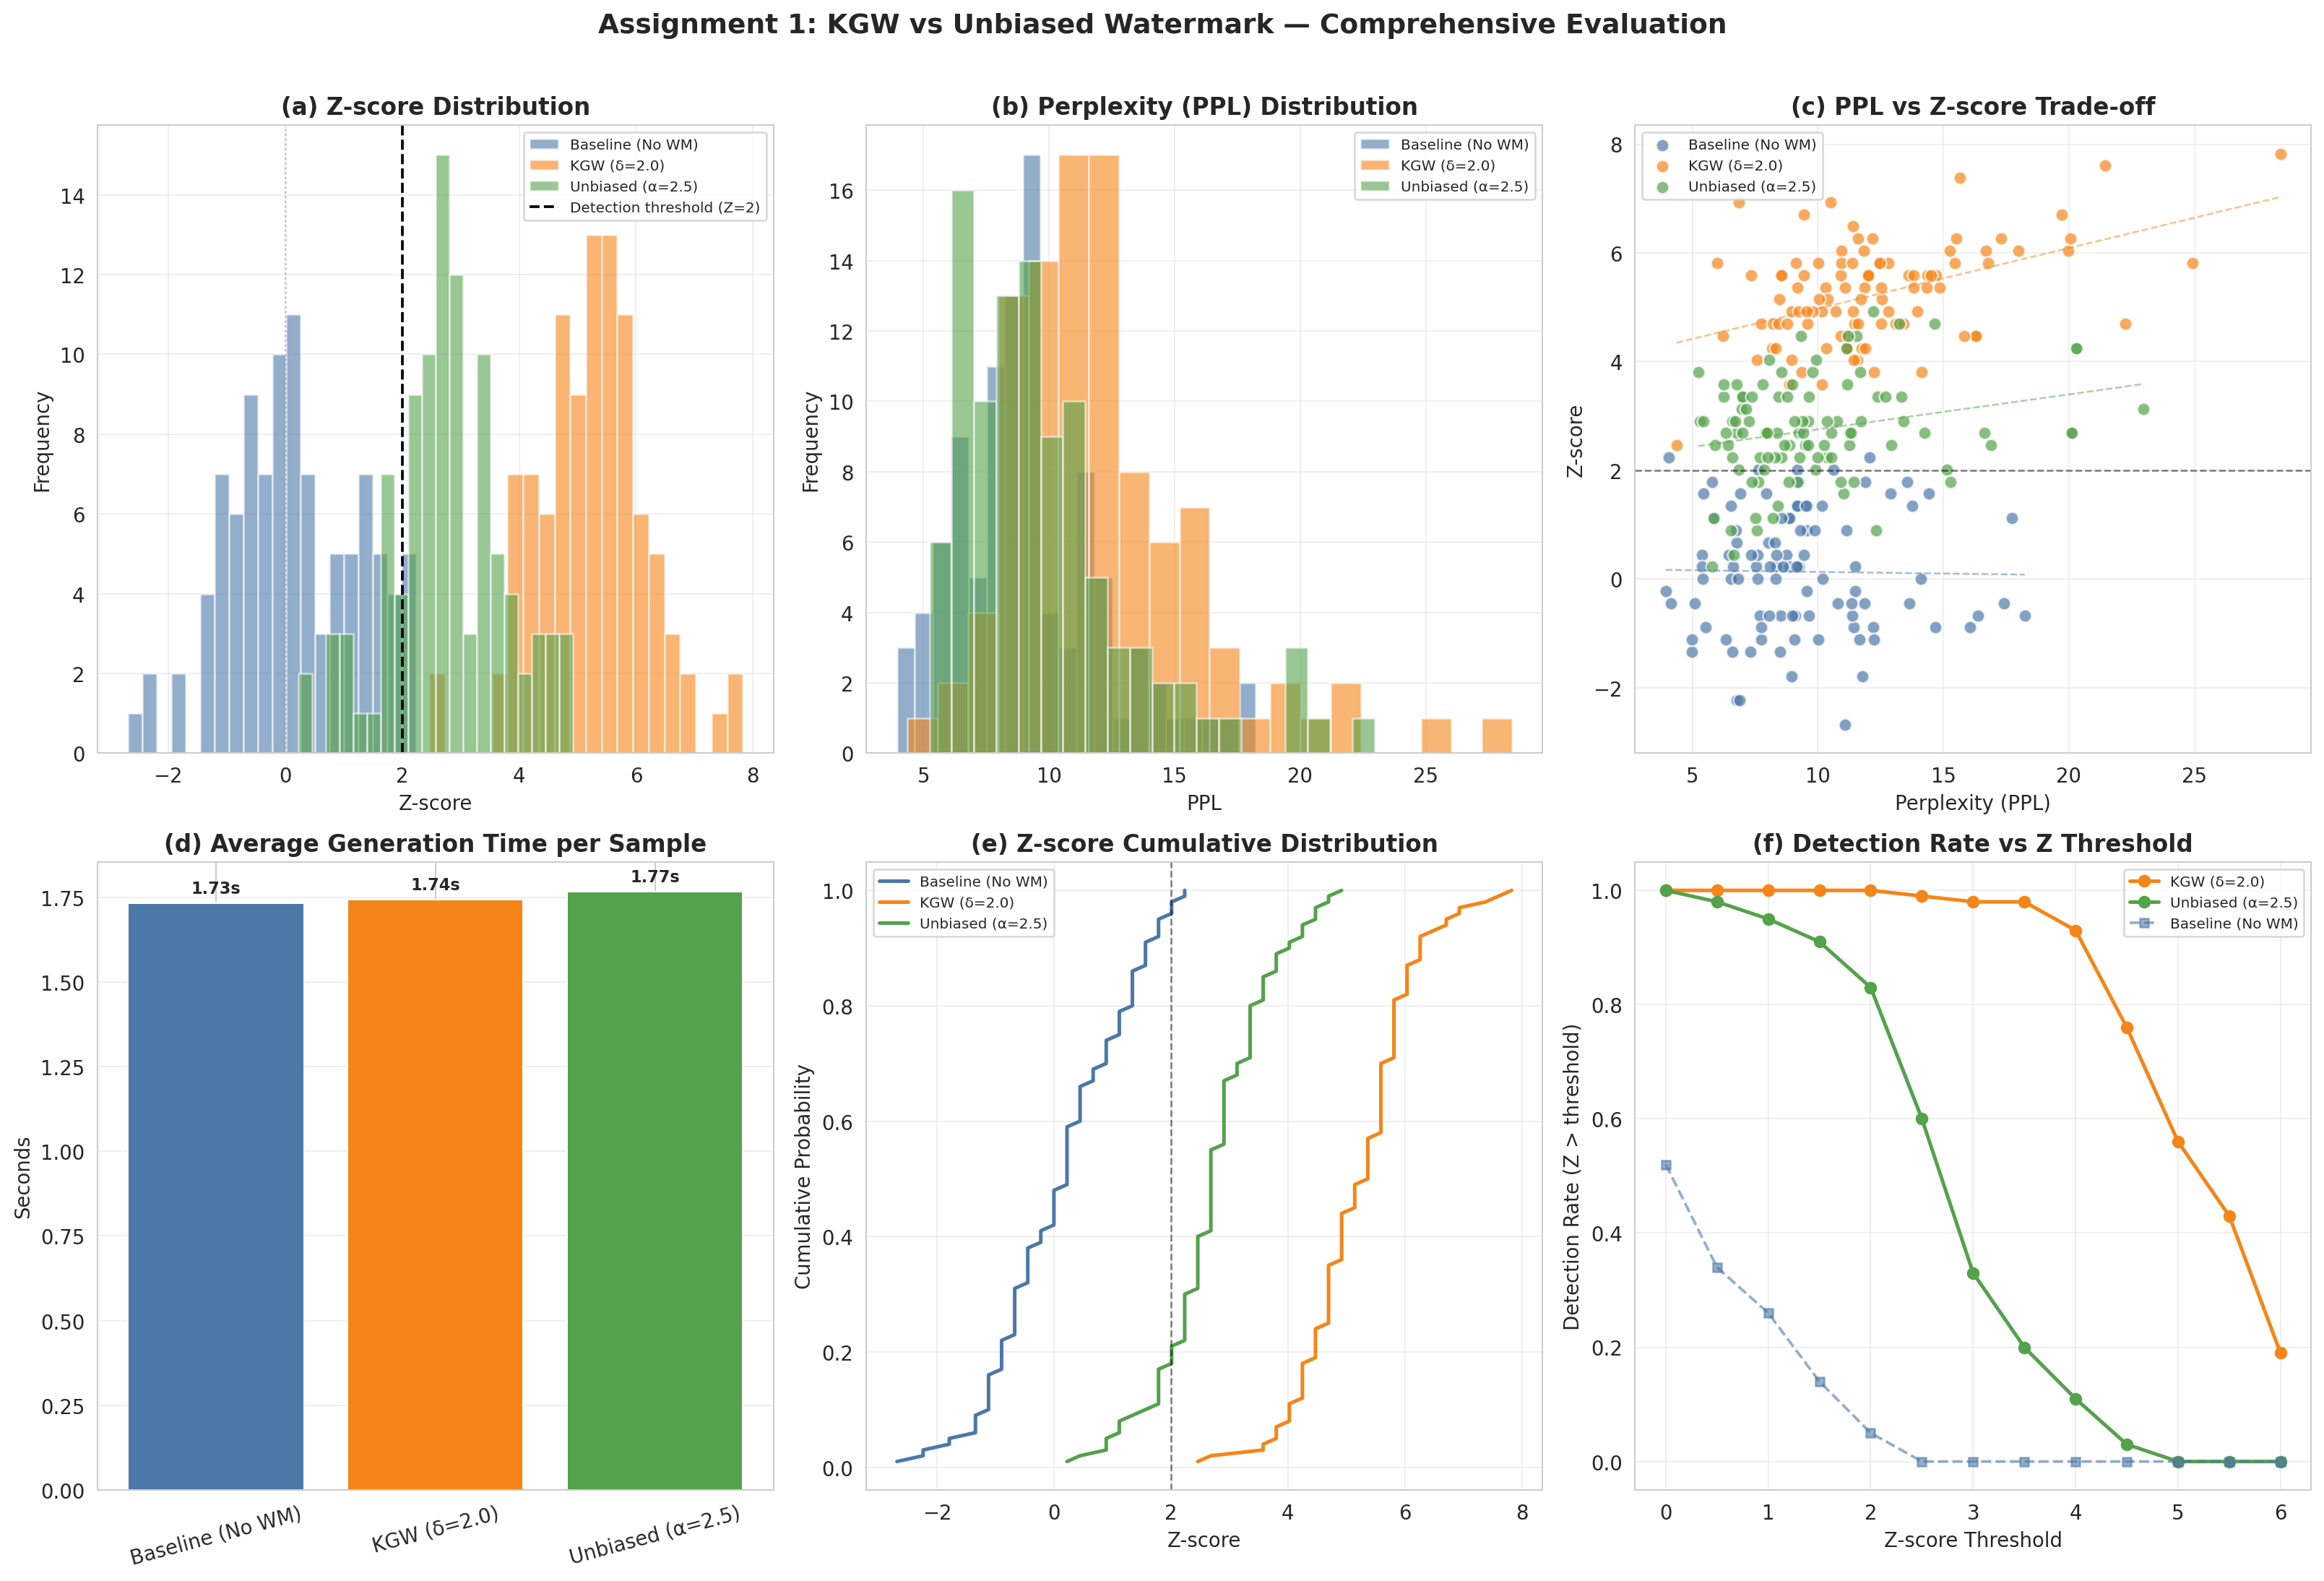
\includegraphics[width=0.95\linewidth]{outputs/assignment1_full_charts.png}
\caption{Detection, quality, and runtime comparison for baseline, KGW, and unbiased watermarking.}
\end{figure}

\subsection{Detection Metrics and Parameter Sensitivity}

Table 2 summarizes representative detection results under different watermark strengths and thresholds.
It compares accuracy, precision, recall, F1, and AUC, which together describe whether a method is both sensitive to watermarked text and conservative on non-watermarked text.

\begin{table}[H]
\centering
\caption{Representative detection results from the systematic evaluation.}
\begin{tabular}{lrrrrrr}
\toprule
Configuration & Threshold & Accuracy & Precision & Recall & F1 & AUC \\
\midrule
KGW $\delta=1.5$ & 2.0 & 0.985 & 0.990 & 0.980 & 0.985 & 0.999 \\
KGW $\delta=2.0$ & 2.0 & 0.995 & 0.990 & 1.000 & 0.995 & 1.000 \\
KGW $\delta=2.5$ & 2.5 & 0.995 & 1.000 & 0.990 & 0.995 & 1.000 \\
KGW $\delta=3.0$ & 3.0 & 1.000 & 1.000 & 1.000 & 1.000 & 1.000 \\
Unbiased $\alpha=3.0$ & 2.0 & 0.905 & 0.955 & 0.850 & 0.899 & 0.970 \\
Unbiased $\alpha=3.5$ & 2.0 & 0.970 & 0.961 & 0.980 & 0.970 & 0.994 \\
\bottomrule
\end{tabular}
\end{table}

Increasing $\delta$ or $\alpha$ monotonically strengthens the watermark signal.
KGW reaches near-perfect or perfect AUC when $\delta$ is at least 1.5, and perfect classification appears for strong settings such as $\delta=3.0$.
The unbiased method requires a larger $\alpha$ to reach comparable recall.
At $z=2$, false positives on human texts remain low; stronger thresholds reduce false positives further but can reduce recall, especially for weaker watermark parameters.

Figure 2 aggregates the systematic evaluation into charts for detection, ROC behavior, quality, runtime, and robustness.
It complements Table 2 by showing trends across more configurations, making the parameter-sensitivity pattern clearer than a small table alone.

\begin{figure}[H]
\centering
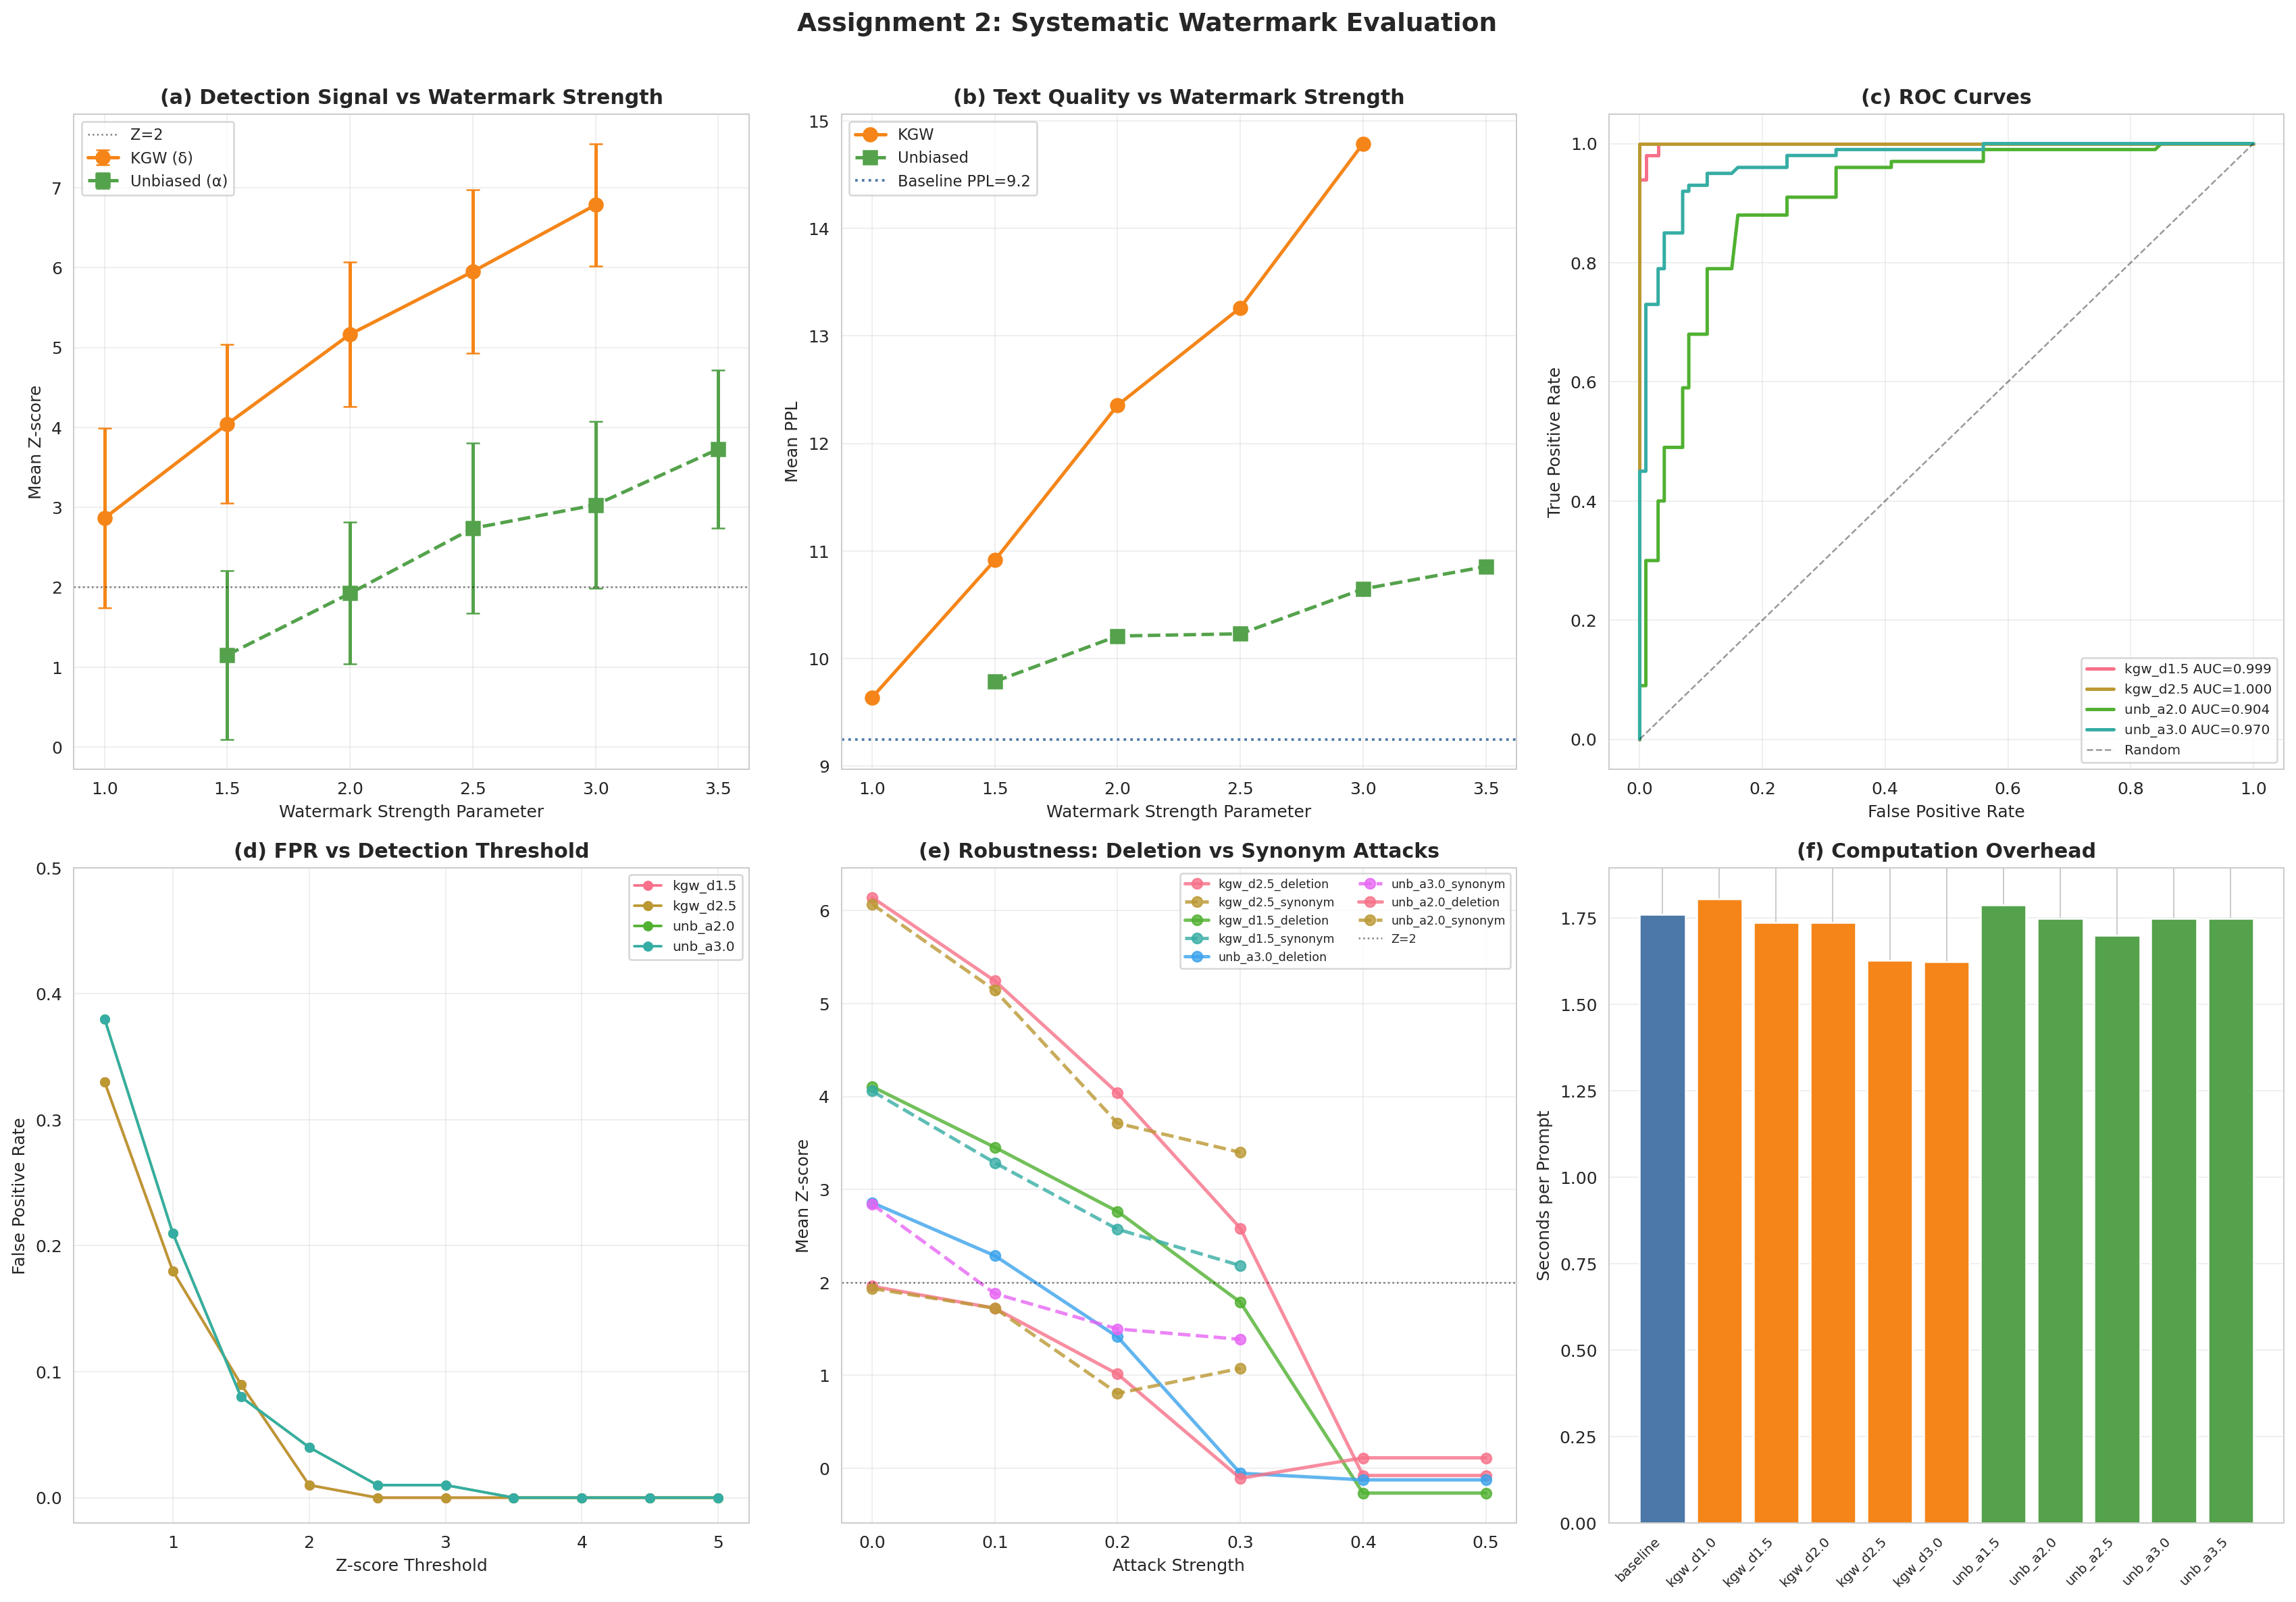
\includegraphics[width=0.95\linewidth]{outputs/assignment2_full_charts.png}
\caption{Systematic detection, ROC, quality, runtime, and robustness analysis.}
\end{figure}

\subsection{Robustness}

Deletion and synonym-substitution attacks reduce z-scores because they remove or alter the token-level evidence used by the detector, which is consistent with prior reliability analyses of watermarked and post-hoc detected AI text \cite{kirchenbauer_reliability2023,sadasivan2023}.
KGW is more robust overall because its additive logit bias creates a stronger initial signal.
In the stored attack traces, KGW with $\delta=2.5$ remains strongly detectable under moderate synonym replacement and light deletion, while weaker KGW and unbiased configurations lose evidence faster.
This confirms a practical tradeoff: stronger watermarks survive attacks better but can increase distributional distortion.

\subsection{Structured Time-Series Watermark}

Table 3 evaluates whether the structured residual watermark changes the visible statistical properties of the generated time series.
The small mean and standard-deviation shifts, very high correlations, and high KS p-value indicate that the watermark is difficult to notice from ordinary distributional summaries.

\begin{table}[H]
\centering
\caption{Quality preservation for structured residual watermarking.}
\begin{tabular}{lrrrr}
\toprule
Metric & Original & Watermarked & Absolute change & Relative change \\
\midrule
Mean & 16.5992 & 16.6545 & 0.0553 & 0.333\% \\
Std & 3.6842 & 3.6867 & 0.0026 & 0.069\% \\
Pearson corr. & 1.0000 & 0.9996 & 0.0004 & 0.043\% \\
Spearman corr. & 1.0000 & 0.9996 & 0.0004 & 0.041\% \\
KS p-value & 1.0000 & 0.9874 & 0.0075 & 0.000\% \\
\bottomrule
\end{tabular}
\end{table}

The structured residual watermark preserves data utility well.
Mean and quantile shifts are below one percent, Pearson and Spearman correlations remain above 0.9995, and the KS p-value remains high at 0.9874.
All 12 payload bits are recovered in the clean setting, with very large absolute bit-level z-scores between 48.88 and 55.06.

Table 4 reports robustness results for the structured residual watermark under four common transformations.
The table shows that aggregation over many records makes the payload robust to additive noise, row deletion, and quantization, while smoothing is the main weakness because it directly suppresses local residual signs.

\begin{table}[H]
\centering
\caption{Structured watermark robustness.}
\begin{tabular}{>{\raggedright\arraybackslash}p{0.16\linewidth}>{\raggedright\arraybackslash}p{0.14\linewidth}>{\raggedright\arraybackslash}p{0.12\linewidth}>{\raggedright\arraybackslash}p{0.11\linewidth}>{\raggedright\arraybackslash}p{0.24\linewidth}}
\toprule
Attack & Max strength & Bit accuracy & Mean $|z|$ & Observation \\
\midrule
Additive noise & 0.18 & 1.000 & 4.39 & Payload recovered. \\
Row drop & 0.60 & 1.000 & 33.23 & Aggregation over many rows is robust. \\
Quantization & Integer rounding & 1.000 & 9.60 & Signal survives coarse rounding. \\
Smoothing & Window 5-15 & 0.750 & 5.04-7.94 & Main weakness: averaging removes residual signs. \\
\bottomrule
\end{tabular}
\end{table}

Figure 3 gives a visual summary of the structured-data experiment.
It links the bit-detection results, quality-preservation metrics, and attack outcomes, making it clear that the proposed residual watermark has strong clean detection and broad robustness but degrades under smoothing.

\begin{figure}[H]
\centering
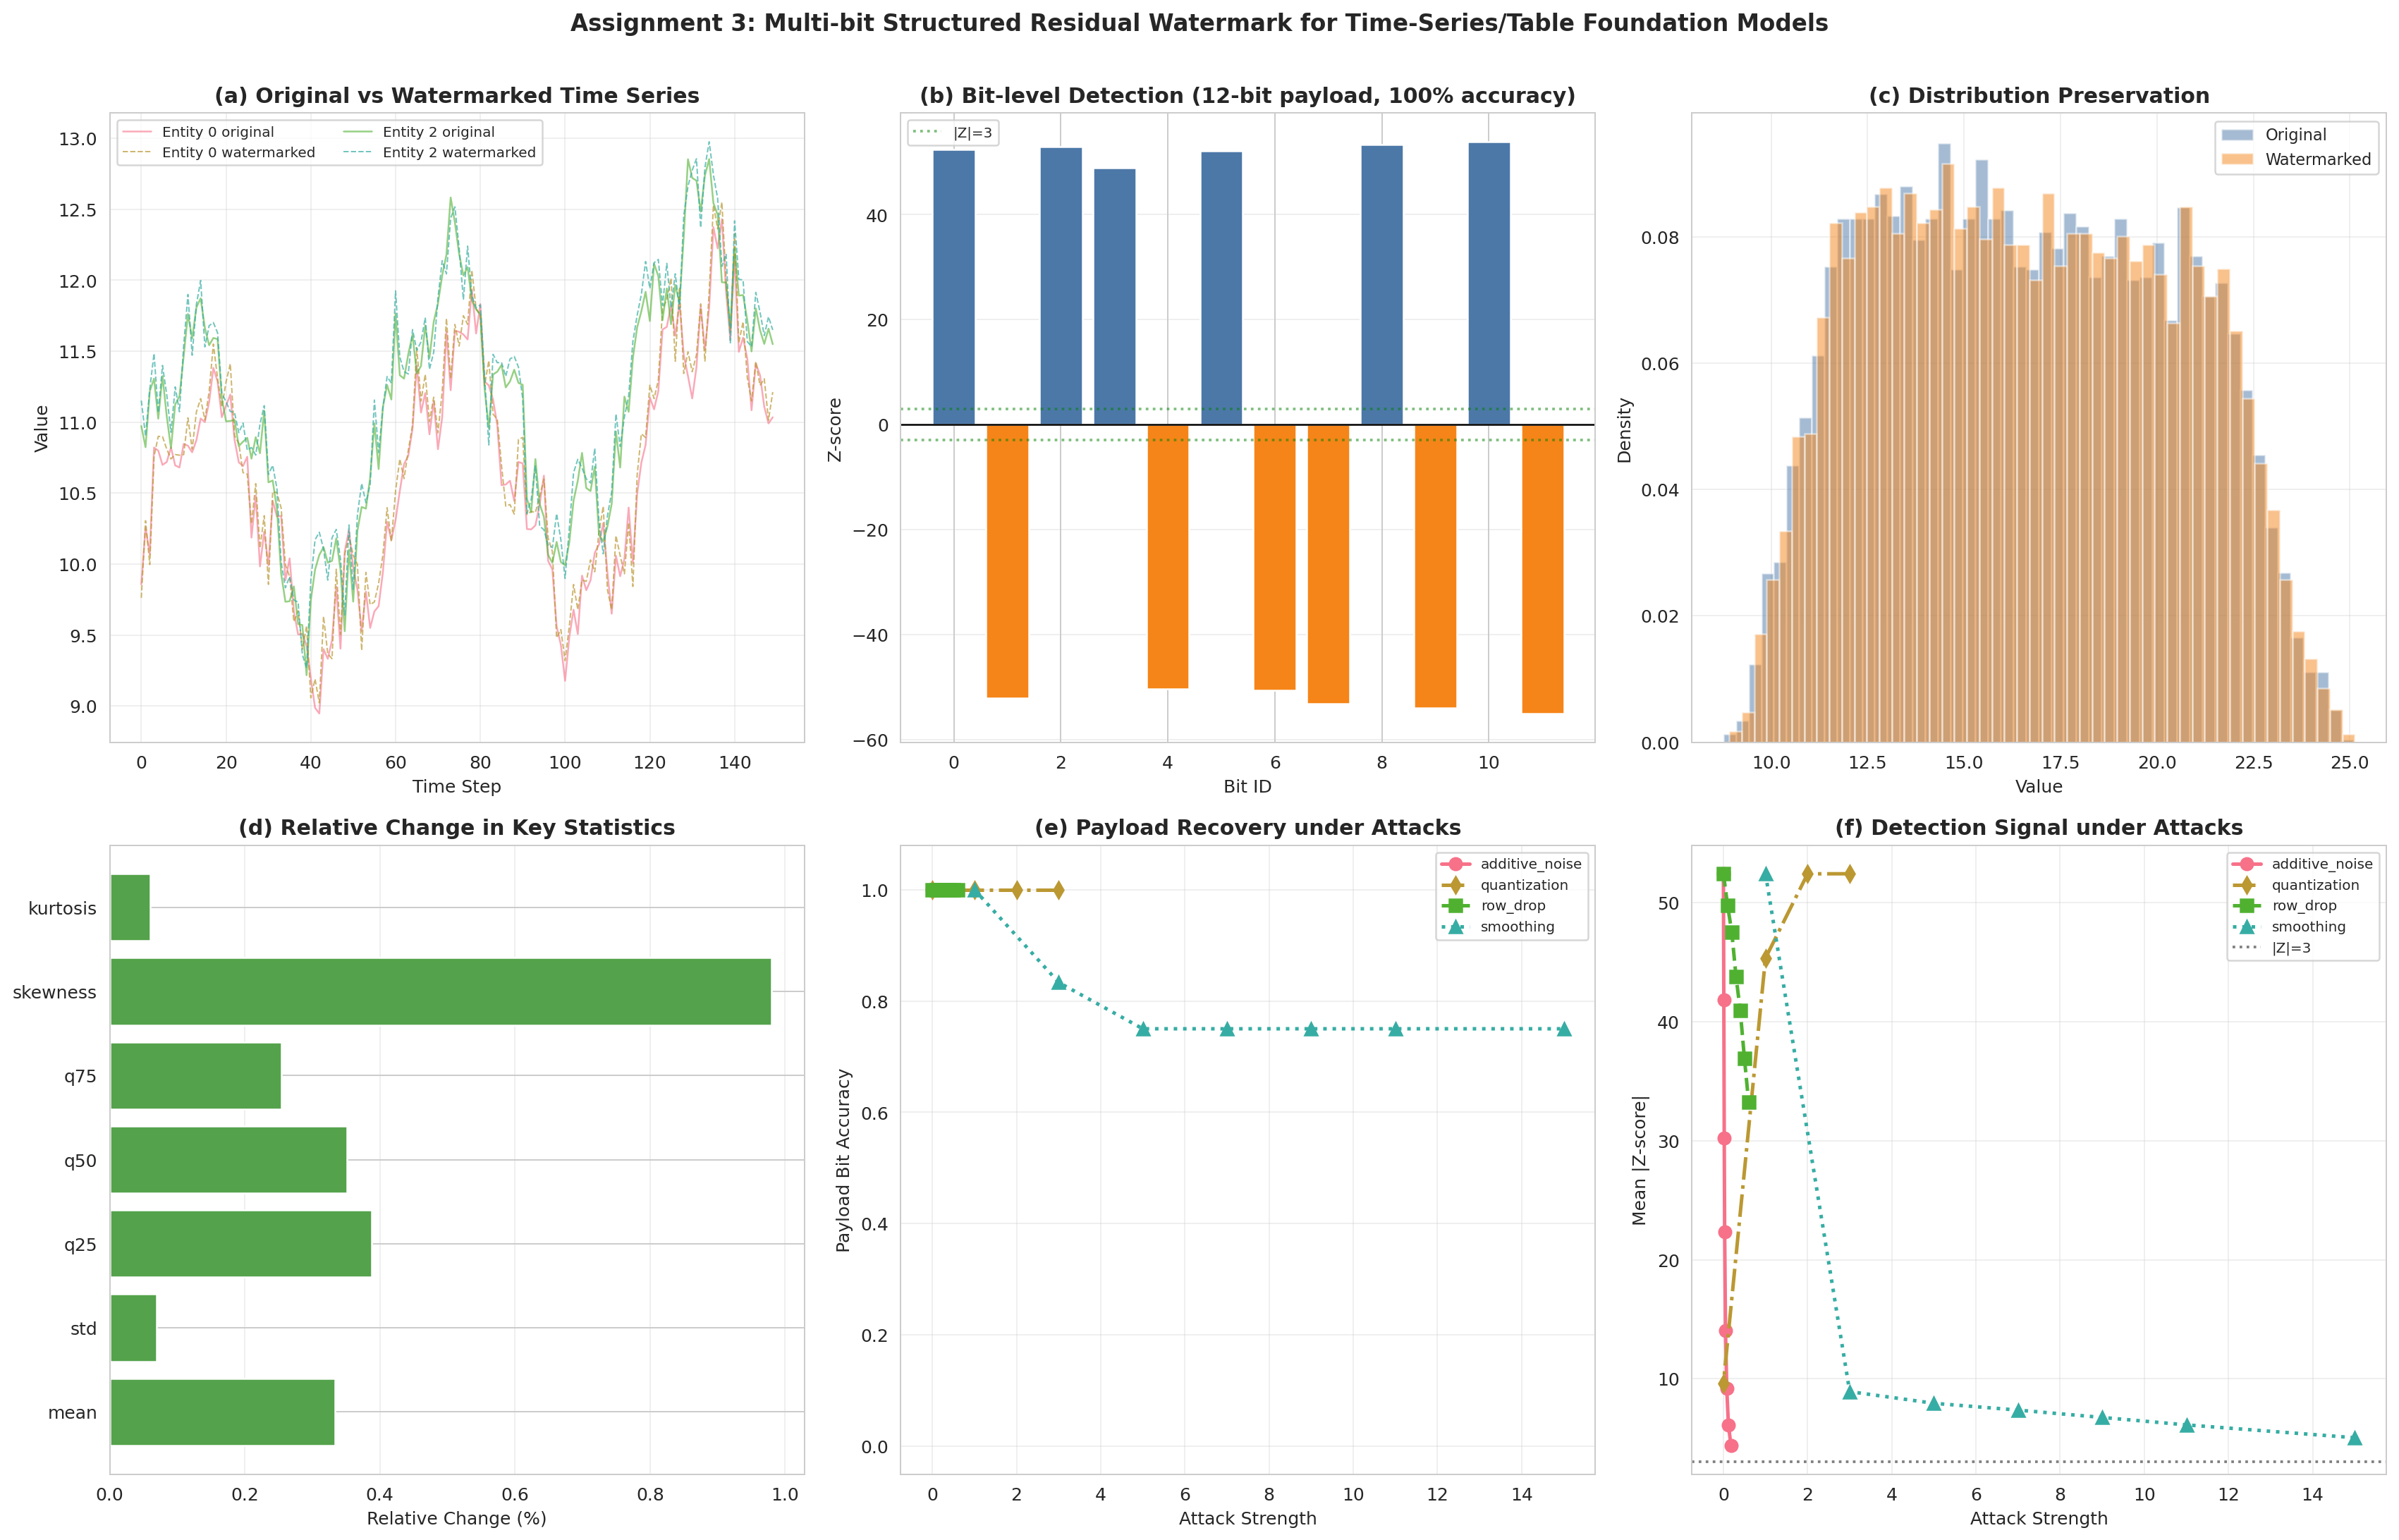
\includegraphics[width=0.95\linewidth]{outputs/assignment3_full_charts.png}
\caption{Structured time-series watermark detection, quality, and attack robustness.}
\end{figure}

\section{Conclusion}

KGW achieved the strongest text watermark detection, with mean $z=5.22$ in the reproduction experiment and AUC up to 1.000 in systematic evaluation.
The unbiased method reduced quality loss, with mean PPL close to baseline, but required stronger parameters to reach high recall.
The proposed structured residual watermark embedded a 12-bit payload into time-series data with minimal statistical distortion and perfect recovery under several common attacks.
These results show that no single watermark setting is optimal for every objective, matching the detection-quality-robustness tradeoff emphasized in previous watermarking studies \cite{kirchenbauer2023,kuditipudi2023,markllm2024}.
KGW is preferable when the priority is confident detection and attack robustness, while the unbiased method is preferable when preserving generation quality is more important and moderate detection confidence is acceptable.
For structured data, residual aggregation can produce extremely strong bit-level evidence while keeping visible statistical changes small, but smoothing attacks are a clear limitation because they specifically suppress high-frequency residual patterns.

A limitation of this project is scale.
The text experiments use a small open-source model and 100 prompts, so the results should be viewed as a controlled reproduction rather than a full deployment study.
Future work should evaluate larger models, longer generations, paraphrase attacks, multilingual prompts, and adaptive attackers who know the detector family but not the secret key, because these factors are repeatedly identified as key deployment risks for AI-text watermarking and detection \cite{kirchenbauer_reliability2023,sadasivan2023}.
Overall, the project demonstrates both the promise and the tradeoffs of watermarking across text and structured-data generation.

\begin{thebibliography}{99}
\bibitem{kirchenbauer2023}
J. Kirchenbauer, J. Geiping, Y. Wen, J. Katz, I. Miers, and T. Goldstein.
\newblock A Watermark for Large Language Models.
\newblock \emph{arXiv preprint arXiv:2301.10226}, 2023.

\bibitem{kirchenbauer_reliability2023}
J. Kirchenbauer, J. Geiping, Y. Wen, M. Shu, K. Saifullah, K. Kong, K. Fernando, A. Saha, M. Goldblum, and T. Goldstein.
\newblock On the Reliability of Watermarks for Large Language Models.
\newblock \emph{arXiv preprint arXiv:2306.04634}, 2023.

\bibitem{kuditipudi2023}
R. Kuditipudi, J. Thickstun, T. Hashimoto, and P. Liang.
\newblock Robust Distortion-free Watermarks for Language Models.
\newblock \emph{arXiv preprint arXiv:2307.15593}, 2023.

\bibitem{sadasivan2023}
V. Sadasivan, A. Kumar, S. Balasubramanian, W. Wang, and S. Feizi.
\newblock Can AI-Generated Text be Reliably Detected?
\newblock \emph{arXiv preprint arXiv:2303.11156}, 2023.

\bibitem{markllm2024}
L. Pan, A. Liu, Z. He, Z. Gao, X. Zhao, Y. Lu, B. Zhou, S. Liu, X. Hu, L. Wen, I. King, and P. S. Yu.
\newblock MarkLLM: An Open-Source Toolkit for LLM Watermarking.
\newblock \emph{arXiv preprint arXiv:2405.10051}, 2024.

\bibitem{survey2024}
Aiwei Liu, Leyi Pan, Yijian Lu, Jingjing Li, Xuming Hu, Xi Zhang, Lijie Wen, Irwin King, Hui Xiong, and Philip S. Yu.
\newblock A Survey of Text Watermarking in the Era of Large Language Models.
\newblock \emph{arXiv preprint arXiv:2312.07913}, 2023.

\bibitem{qwen25}
Qwen.
\newblock Qwen2.5 Technical Report.
\newblock \emph{arXiv preprint arXiv:2412.15115}, 2024.
\end{thebibliography}

\end{document}
